    \chapter{Introduction aux idées fondamentales}

                Le début du $XX^e$ siècle a vu naître avec lui la physique quantique, tirant son nom de la quantification des grandeurs observées dans un système physique au lieu des traditionnels continuums de la physique classique. En particulier, c'est l'introduction du quantum d'énergie par Max Planck en 1901 qui permettra de résoudre le problème de la \textit{catastrophe ultraviolette}, et qui conduira de nombreux physiciens tels que Niels Bohr, Albert Einstein ou encore Louis de Broglie à développer de nouveaux modèles dans le cadre de la \textit{théorie des quanta}. Sur cette base, des phénomènes comme la lumière alors décrits de façon purement ondulatoire trouveront une nature corpusculaire tandis que des objets tels que l'électron, décrits comme purement matériels, seront traités à la fois comme onde et particule. Ce concept est nommé la \textit{dualité onde-corpuscule} et servira de point de départ à la description des particules en mécanique quantique dans la première partie de ce chapitre. La seconde partie sera dédiée à une présentation des grandes idées de la mécanique quantique non-relativiste permettant de décrire l'évolution dans le temps d'un système quantique. Enfin les troisième et quatrième parties tenteront de présenter le cheminement des physiciens pour unifier la mécanique quantique à la relativité restreinte d'Albert Einstein \cite{Einstein1905} afin d'aboutir à la théorie quantique des champs, base essentielle de la physique des particules moderne. D'autres éléments permettant une introduction aux concepts fondamentaux traités dans cette thèse seront également présentés.
                
        \section{Description quantique des particules}
        
            Avec la découverte du photon, particule de lumière, la quantification de l'énergie est devenue indispensable pour la compréhension de certaines observations physiques comme les spectres d'absorption et d'émission des atomes qui présentent des raies fines et discrètes. Ce phénomène traduit la possibilité pour un atome d'absorber ou d'émettre des photons uniquement à des longueurs d'onde précises. Cela implique qu'un photon doit posséder une énergie correspondante à l'écart entre deux niveaux d'énergie $E_i$ et $E_j$ de l'atome pour être absorbé, et qu'un photon émit possédera une énergie égale à l'écart entre deux niveaux selon la formule : 
            
            \begin{equation}
                h\nu_{ij}=|E_i-E_j|,
            \end{equation}
            
        où $h\simeq6.62\times10^{-34}$ J.s est une constante appelée \textit{constante de Planck} et $\nu_{ij}$ est la fréquence d'un photon. En 1923, Louis de Broglie, inspiré par l'hypothèse de Max Planck, proposa  que \textit{<<les corpuscules matériels, tout comme les photons, peuvent avoir un aspect ondulatoire>>}. L'expérience de Davisson et Germer \cite{Germer1927} prouvera cette hypothèse en 1927 en montrant un comportement des électrons analogue à celui de la lumière par diffraction. Dès lors, on associera à tout corpuscule matériel d'énergie $E$ et d'impulsion $\vb{p}$ les relations de Planck-Einstein introduites pour le photon en 1924 après la découverte de \textit{l'effet Compton} \cite{Compton1923} :
            
            \begin{equation}
                \left\{
                    \begin{array}{ll}
                        E & = h\nu \\
                        \vb{p} & = \hbar\vb{k},
                    \end{array}
                \right.
            \end{equation}

            avec $\hbar=h/2\pi$ et $\vb{k}$ le vecteur d'onde, d'où découle l'expression d'une longueur d'onde d'après la relation de Louis de Broglie :
            
            \begin{equation}
                \lambda=\frac{2\pi}{|\vb{k}|}=\frac{h}{|\vb{p}|}.
            \end{equation}
            
        Désormais la nature ondulatoire d'un corpuscule devient indissociable de sa nature matérielle. Il est également intéressant de noter que la petite valeur de la constante de Planck interdit l'observation du phénomène ondulatoire de la matière au-delà des échelles d'énergie de \textit{l'infiniment petit}.
        
        \section{Mécanique quantique non-relativiste}
        
         D'après les éléments apportés par le paragraphe précédent, une particule libre peut être décrite comme un état quantique $\ket{\psi(t)}$ dépendant du temps $t$, à travers un objet de nature ondulatoire appelé fonction d'onde et noté $\psi(\vb{x},t)$, correspondant à la projection de l'état quantique $\ket{\psi(t)}$ sur une base $\ket{\vb{x}}$ de l'espace :
        
        \begin{equation}
            \psi(\vb{x},t)=\bra{\vb{x}}\ket{\psi(t)}\propto Ne^{i(\vb{p}.\vb{x}-Et)},
            \label{onde}
        \end{equation}
            
        où $N$ est une constante de normalisation. La définition de cet objet veut que toute information sur un état quantique soit contenue dans sa fonction d'onde. Ainsi la première conséquence sera que la notion de trajectoire telle qu'elle est entendue au sens classique doit être abandonnée au profit d'une amplitude de probabilité de présence en un point donné de l'espace. D'autre part, l'accès à certaines grandeurs comme l'impulsion ou l'énergie d'une particule se fait à travers des opérateurs $\hat{A}$ agissant sur la fonction d'onde de manière à retourner une grandeur $a$ :
        
        \begin{equation}
            \hat{A}\psi(\vb{x},t)=a\psi(\vb{x},t).
        \end{equation}
        
        On dit alors que $\psi(\vb{x},t)$ est un état propre de l'opérateur $\hat{A}$, de valeur propre $a$, et cette grandeur correspondra à une observable physique lorsque sa valeur sera purement réelle. Dans le cas de l'impulsion et de l'énergie, il est possible d'introduire respectivement les opérateurs $\hat{\vb{p}}$ et $\hat{E}$ :
        
        \begin{equation}
            \hat{\vb{p}} = -i\grad \quad \mbox{et } \quad
            \hat{E} = i\pderivative{t},
            \label{ops}
        \end{equation}

        de sorte à obtenir en utilisant l'expression \ref{onde} de la fonction d'onde :
        
        \begin{equation}
            \left\{
                \begin{array}{ll}
                    \hat{\vb{p}}\psi(\vb{x},t)=\vb{p}\psi(\vb{x},t) \\
                    \hat{E}\psi(\vb{x},t)=E\psi(\vb{x},t).
                \end{array}
            \right.
        \end{equation}       
        
        Par analogie à la mécanique classique, où l'énergie totale d'un système est donnée par la somme de l'énergie cinétique $T$ et de l'énergie potentielle $V$ à travers l'Hamiltonien $H=T+V$, il est possible de définir un opérateur Hamiltonien quantique pour une particule de masse $m$ :
        
        \begin{equation}
                \hat{H}=\frac{\hat{\vb{p}}^2}{2m}+\hat{V}=-\frac{1}{2m}\laplacian + \hat{V}.
        \end{equation}
        
        L'application de l'opérateur Hamiltonien sur la fonction d'onde donne lieu à la célèbre équation de Schrödinger dépendante du temps qui permet de décrire à tout instant l'évolution de $\psi(\vb{x},t)$ :
        
        \begin{equation}
        \boxed{
            i\pdv{\psi(\vb{x},t)}{t}=\hat{H}\psi(\vb{x},t).
        }
        \end{equation}
        
        D'après l'opérateur énergie introduit plus tôt, on remarque alors que si la fonction d'onde $\psi_i(\vb{x},t)$ est un état propre de l'opérateur Hamiltonien on obtient naturellement :
        
        \begin{equation}
            \hat{H}\psi_i(\vb{x},t)=E_i\psi_i(\vb{x},t).
        \end{equation}
        
        Comme mentionné plus tôt, la fonction d'onde contient toutes les informations d'un système quantique et peut ainsi être utilisée pour définir une densité de probabilité de présence. Si la valeur $\psi^*(\vb{x},t)\psi(\vb{x},t)\dd[3]{\vb{x}}$ est associée à la probabilité de trouver une particule dans le volume infinitésimal $\dd[3]{\vb{x}}$, alors cette densité de probabilité est définie selon :
        
        \begin{equation}
            \rho(\vb{x},t)=\psi^*(\vb{x},t)\psi(\vb{x},t).
        \end{equation}
        
        L'évolution temporelle de $\rho(\vb{x},t)$ permet également de définir un courant de probabilité $\vb{j}(\vb{x},t)$, en considérant que si la densité de probabilité au sein d'un volume varie alors il existe un courant de probabilité à travers les parois de ce volume :
        
        \begin{equation}
            \pdv{t}\int_V\rho\dd{V}=-\int_S\vb{j}\vdot \dd{\vb{S}}=-\int_V\grad\vdot\vb{j}\dd{V}.
            \label{div}
        \end{equation}

        Le dernier terme de \ref{div} est obtenu grâce au théorème de la divergence, et cette équation étant valide pour tout volume arbitraire il est possible d'écrire l'équation de continuité suivante :

        \begin{equation}
            \grad\vdot\vb{j}+\pdv{\rho}{t}=0.
        \end{equation}

        L'équation de Schrödinger pour une particule libre, c'est à dire sans terme de potentiel, permet de définir la forme du courant $\vb{j}$ en écrivant :

        \begin{equation*}
        \begin{split}
        i\pdv{\rho}{t} & =i\pdv{t}(\large\psi^*\psi) \\
         & = i\Biggl(\pdv{\psi^*}{t}\psi + \psi^*\pdv{\psi}{t}\Biggr) \\
         & = -\frac{1}{2m}(\psi^*\laplacian\psi-\psi\laplacian\psi^*) \\
         & = -\frac{1}{2m}\grad\vdot(\psi^*\grad\psi-\psi\grad\psi^*) \\
        \end{split}
        \end{equation*}

        Soit :

        \begin{equation*}
            \vb{j} = \frac{1}{2im}(\psi^*\grad\psi-\psi\grad\psi^*). \\
        \end{equation*}

        En résumé, la densité de probabilité et le courant de probabilité exprimé en fonction de l'expression de la fonction d'onde \ref{onde} peuvent s'écrire :

        \begin{equation}
            \boxed{
            \rho=\psi^*\psi \quad \mbox{et} \quad \vb{j}=|N|^2\frac{\vb{p}}{m}.
            }
        \end{equation}
        
        Pour tout opérateurs $\hat{A}$ et $\hat{B}$ il également possible de définir une relation de commutation 
        
        \begin{equation}
            [\hat{A},\hat{B}]=\hat{A}\hat{B}-\hat{B}\hat{A},
        \end{equation}
        
        pour laquelle on dira que $\hat{A}$ et $\hat{B}$ commutent lorsque $[\hat{A},\hat{B}]=0$, et ne commutent pas le cas échéant. Cette relation a de fortes implications en mécanique quantique, puisqu'elle détermine la possibilité ou non de mesurer simultanément deux observables d'un état quantique. À titre d'exemple, la non-commutation des opérateurs de position et d'impulsion permet d'illustrer le principe d'incertitude de Heisenberg selon lequel il est impossible de connaître simultanément de façon précise la vitesse et la position d'une particule. 
    
        \section{Vers une théorie quantique relativiste}
        \label{verslarelat}
        
         Le début du $XX^e$ siècle marque également la naissance de la relativité restreinte par Albert Einstein permettant de décrire des systèmes ayant une vitesse non négligeable devant celle de la lumière. Selon cette théorie, la vitesse de la lumière est une constante dans tout référentiel galiléen et implique qu'une cause entraîne toujours un effet dans un délai minimal nécessaire à la lumière pour parcourir la distance entre la cause et l'effet dans ce qui est nommé \textit{principe de causalité}. Les objets relativistes sont quant à eux décrits dans un espace à quatre dimensions appelé \textit{espace-temps de Minkowski} grâce à des quadrivecteurs dans lesquels le temps devient une composante à part entière aux côtés des trois coordonnées spatiales $(x,y,z)$ de l'espace Euclidien. Ces objets peuvent également subir des transformations de coordonnées grâce aux transformations de Lorentz, à l'origine des effets de dilatation temporelle de la relativité restreinte. Certaines quantités telle que la masse en physique des particules sont inchangées par ces transformations, elles sont alors \textit{invariantes de Lorentz}. L'équation de Schrödinger, qui comporte un terme de dérivation temporelle au premier ordre tandis que le terme de dérivation spatiale est au second, n'est pas invariante de Lorentz et est donc incompatible avec la relativité restreinte d'Einstein. En revanche des systèmes physiques tels que l'atome d'hydrogène représenté par un électron plongé dans un potentiel coulombien, induit par le proton, ne peuvent être décrits de manière complète sans inclure des effets relativistes. Les premiers travaux pour concilier relativité et mécanique quantique seront réalisés indépendamment par Oskar Klein et Walter Gordon en 1926. En effet, il est possible à partir de la forme relativiste de la relation entre énergie et impulsion 
        
        \begin{equation}
            E^2=\vb{p}^2+m^2,
            \label{Eprelation}
        \end{equation}

        de construire une équation relativiste en remplaçant chaque terme par un opérateur tel qu'introduit dans l'équation \ref{ops} et agissant sur une fonction d'onde $\psi(\vb{x},t)$. On obtient alors l'équation de Klein-Gordon :
        
        \begin{equation}
        \boxed{
            (\partial^{\mu}\partial_{\mu}+m^2)\psi(\vb{x},t)=0
        ,}
        \label{KG}
        \end{equation}
        
        avec $$\partial^{\mu}\partial_{\mu}\equiv\pdv[2]{t}-\pdv[2]{x}-\pdv[2]{y}-\pdv[2]{z}.$$
        
        Comme pour l'équation de Schrödinger, il est possible de définir une densité et un courant de probabilité :

        \begin{equation}
        \boxed{
            \rho=2|N|^2E \quad \mbox{et} \quad \vb{j}=2|N|^2\vb{p}.
        }
        \end{equation}
        
        Malgré une réussite apparente de joindre la relativité d'Einstein à la mécanique quantique, cette équation apporte également une densité de probabilité de présence négative dépourvue de sens physique aux solutions d'énergie négative. Ces résultats ont amené Paul Dirac en 1928 à rechercher à son tour une équation relativiste, qui face aux conclusions précédentes, devra être dérivée d'ordre un à la fois d'espace et de temps et de forme générale :
        
        \begin{equation}
            \hat{E}\psi=(\vb*{\alpha}\vdot\vb{\hat{p}}+\beta m)\psi.
            \label{dirac1}
        \end{equation}
        
        Il est également nécessaire, pour décrire correctement des objets relativistes, que les solutions de cette équation obéissent à la relation relativiste entre l'énergie et l'impulsion \ref{Eprelation}. Ainsi l'équation proposée par Dirac doit être compatible avec l'équation de Klein-Gordon. Il est alors possible de montrer à partir de cette condition que les objets $\vb*{\alpha}=(\alpha_x, \alpha_y, \alpha_z)$ et $\beta$ constituent un ensemble de  quatre matrices de dimension quatre agissant sur une fonction d'onde particulière à quatre composantes appelée \textit{spineur de Dirac} :
  
        \[
            \psi = 
            \begin{pmatrix}
                \psi_1 \\
                \psi_2 \\
                \psi_3 \\
                \psi_4
            \end{pmatrix}
        ,\]
        
        et que la forme la plus simple pour $\vb*{\alpha}$ et $\beta$ se retrouve dans la représentation de Dirac-Pauli avec :
        
        \[
            \alpha_i = 
            \mqty(0 && \sigma_i \\ \sigma_i && 0)
            \quad
            \mbox{ et }
            \quad
            \beta = 
            \mqty(I && 0 \\ 0 && -I)
        ,\]
        
        où $i=x,y,z$, avec $\sigma_i$ représentant chacune une des trois matrices de Pauli :
        
        \[
            \sigma_x = 
            \mqty(0 && 1 \\ 1 && 0)
            \mbox{, }
            \quad
            \sigma_y = 
            \mqty(0 && -i \\ i && 0)
            \mbox{, }
            \quad
            \sigma_z = 
            \mqty(1 && 0 \\ 0 && -1)
        \]
        
        et où $I$ est la matrice unité de dimension deux. \\
        
        On retrouvera plus souvent l'équation de Dirac sous sa forme dite covariante :
        
        \begin{equation}
        \boxed{
            (i\gamma^{\mu}\partial_{\mu}-m)\psi(\vb{x},t)=0,
        }
        \label{dirac2}
        \end{equation}
        
        avec
        
        $$
        \begin{array}{ll}
            \gamma^{\mu}\partial_{\mu} & \equiv\gamma^0\pdv{t}+\gamma^1\pdv{x}+\gamma^2\pdv{y}+\gamma^3\pdv{z} \\
            & \\
            & \equiv\beta\pdv{t}+\beta\sigma_x\pdv{x}+\beta\sigma_y\pdv{y}+\beta\sigma_z\pdv{z}.
        \end{array}
        $$

        Finalement l'expression de la densité et du courant de probabilité est donnée par :

        \begin{equation}
            \boxed{
            \rho=\psi^{\dag}\psi \quad \mbox{et} \quad \vb{j}=\psi^{\dag}\vb*{\alpha}\psi,
            }
        \label{probdirac}
        \end{equation}

        où $\psi^{\dag}=(\psi^*)^T$ est le conjugué hermitien de $\psi$. \\
        
        Bien que cette nouvelle équation semble effectivement compatible avec la relativité restreinte, elle autorise également l'énergie de l'électron à prendre des valeurs négatives dont les physiciens peineront à justifier l'existence. Paul Dirac a alors tenté dans un premier temps de décrire l'existence d'une $\textit{mer}$ constituée d'électrons virtuels occupants de manière discrète tous les niveaux d'énergie allant de l'infini négatif à une valeur maximale appelée $\textit{niveau de la mer}$, où un électron quittant cette mer laisserait derrière lui un <<trou>> dont l'énergie serait positive. Devant les incohérences de cette théorie et après une tentative échouée d'établir un lien avec le proton, il postulera finalement en 1931 l'existence du positron, jumeau d'anti-matière de l'électron, découvert l'année suivante en chambre à brouillard par Carl David Anderson \cite{Anderson1932}. \\
        
        Il est également intéressant de noter au sujet de l'équation de Dirac sa capacité à intégrer naturellement dans son formalisme les degrés de liberté supplémentaires du spin de l'électron, notion prédite quelques années plus tôt. En effet, certaines observations physiques du début du siècle telles que la levée de dégénérescence des niveaux d'énergie d'un atome plongé dans un champ magnétique et leur structure hyperfine, ou encore les résultats de l'\textit{expérience de Stern et Gerlach} \cite{Gerlach1922}, ont trouvé une explication lors de l'introduction du spin en 1925 par Samuel Goudsmit et George Uhlenbeck \cite{Uhlenbeck1925}. Bien que d'abord vu comme une rotation de l'électron sur lui-même, il s'agit en réalité d'un degré de liberté supplémentaire sans équivalent classique davantage lié à des propriétés magnétiques que mécaniques. Le spin de l'électron a par la suite été formalisé par Wolfgang Pauli en 1927 sous forme d'opérateurs agissant sur la fonction d'onde et constitués des trois matrices de Pauli présentées plus tôt. Dans ce formalisme, l'opérateur de spin $\hat{S}$ est introduit comme un opérateur vectoriel composé des trois composantes spatiales $\hat{S_x}, \hat{S_y}, \hat{S_z}$ ne commutant pas entre elles mais qui commutent individuellement avec $\hat{S}$. En d'autres termes, la mécanique quantique autorise uniquement la mesure simultanée du spin total d'une particule et de sa projection sur une des trois directions de l'espace, la connaissance de sa valeur dans les autres directions étant alors perdue.
        
        \section{L'interaction par la théorie des champs}
        \label{sectionQFT}
        
        Du côté de la physique classique, la théorie du champ électromagnétique découlant directement des équations de Maxwell était déjà une excellente intégration de la relativité restreinte dans un modèle physique. Elle permet notamment de décrire avec succès les interactions de la matière chargée et le comportement du rayonnement électromagnétique. Dans une première tentative de quantification de l'électromagnétisme, Dirac tenta de décrire de manière séparée la matière chargée par le formalisme ondulatoire de Schrödinger et le rayonnement par la propagation d'une onde quantifiée associée au photon. De ce point de vue, la mécanique quantique est alors incapable d'unir la vision d'une particule chargée a priori éternelle à celle d'un photon éphémère capable d'être créé par émission puis annihilé par absorption. Ce problème se verra résolu de manière naturelle, mais non sans difficulté, par le développement pendant plus de 10 ans de la théorie quantique des champs (QFT, \textit{Quantum Field Theory}) selon laquelle toute particule peut être associée à un champ. Dans ce nouveau formalisme les opérateurs de création et d'annihilation, dénotés $\hat{a}^{\dag}_k$ et $\hat{a}_k$ respectivement, sont introduits dans le but d'agir sur un champ donné afin de créer ou annihiler un quanta d'énergie représenté par une particule associée à ce champ. Dans ce cadre, les solutions de l'équation de Klein-Gordon \ref{KG} représentent des champs scalaires qui, une fois soumis à l'action de l'opérateur de création, donnent naissance à des particules sans spin appelées bosons scalaires, tandis que les solutions de l'équation de Dirac \ref{dirac1} donnent naissance à des fermions de spin $\sfrac{1}{2}$ tels que l'électron. D'autres champs de type vectoriels sont quant à eux capables de produire des particules de spin 1 appelées bosons vecteurs à trois degrés de liberté de spin, soit un de plus que les fermions, à l'exception du photon qui possède seulement deux états de polarisation car non massif. \\
        
        Il reste toutefois à décrire la façon dont les différentes particules sont susceptibles d'interagir entre elles afin de produire des processus physiques observables expérimentalement. La mécanique quantique décrit la transition d'un état initial vers un état final dans le cadre de la théorie des perturbations, selon laquelle une particule se diffuse dans un potentiel extérieur en échangeant une partie de son impulsion. Cette vision est néanmoins incomplète sur deux aspects fondamentaux : elle fait intervenir le concept d'interaction sans fournir la description d'un quelconque médiateur, et viole la causalité dans le sens où si une autre particule est ajoutée au système son potentiel prendrait effet dans la perturbation partout et instantanément. Dans le cadre de la QFT ces aspects sont couverts en donnant à des particules porteuses de force le rôle de médiatrices, ce qui ne viole pas la causalité puisque ces échanges sont limités par la vitesse de ces particules nécessairement inférieure à celle de la lumière. Prenons le cas d'une interaction entre deux électrons notés $e_1$ et $e_2$ durant laquelle se produit un transfert d'impulsion par échange d'une particule $X$. Il serait possible a priori de décrire ce processus de sorte que $e_1$ soit responsable de l'émission de $X$ à un instant $t_1$ qui sera ensuite absorbée par $e_2$ à un instant ultérieur $t_2$, ou au contraire que $e_2$ soit responsable de l'émission à $t_1$, et $e_1$ de l'absorption à $t_2$. Ces deux modes d'action peuvent en réalité d'un point de vue mathématique être sommés et condensés en un seul diagramme appelé \textit{diagramme de Feynman} (fig.\ref{sumfeynman}). Inventés par Richard Feynman dans les années 1940, ces diagrammes sont une représentation graphique qui au-delà de leur aspect simple contiennent toute la complexité calculatoire de la théorie quantique des champs. Ils permettent notamment d'illustrer la somme des différentes  chronologies d'un processus physique comme vu dans l'exemple précédent, ainsi que toutes les combinaisons de spin des particules impliquées. \\
        
        \begin{figure}
            \centering
            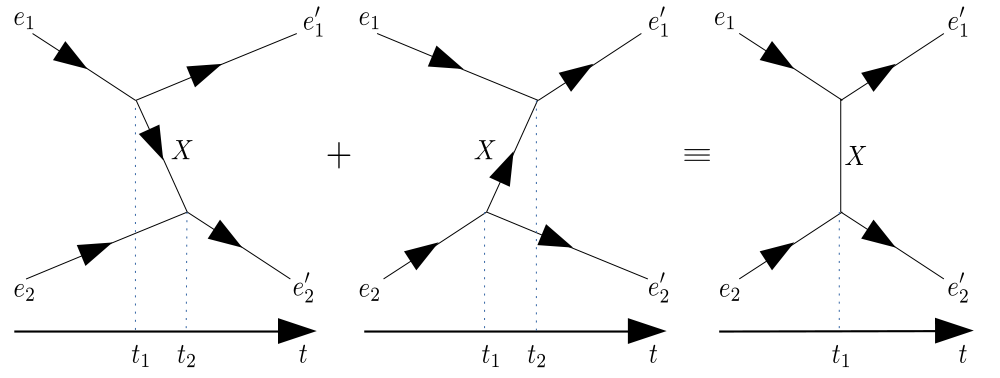
\includegraphics[scale=0.28]{Chapitre1/Images/sumfeynman.png} 
            \caption{Différentes chronologies de l'interaction entre $e_1$ et $e_2$ et représentation du diagramme de Feynman associé.}
        \label{sumfeynman}
        \end{figure}
        
        La figure \ref{bhabha} illustre un exemple réel d'interaction entre un électron et un positron appelée diffusion Bhabha. Ce processus fait intervenir l'échange d'un photon entre une paire électron/positron (e$^+$/e$^-$) dans le cadre de la théorie quantique de l'électromagnétisme (QED, \textit{Quantum Electrodynamics}), première théorie basée sur la QFT datant de la fin des années 1940. On peut alors écrire le diagramme de Feynman associé de deux façons, la première étant une annihilation donnant naissance à une nouvelle paire (voie $s$), et la seconde une diffusion élastique classique (voie $t$). \\
        
        \begin{figure}
            \centering
            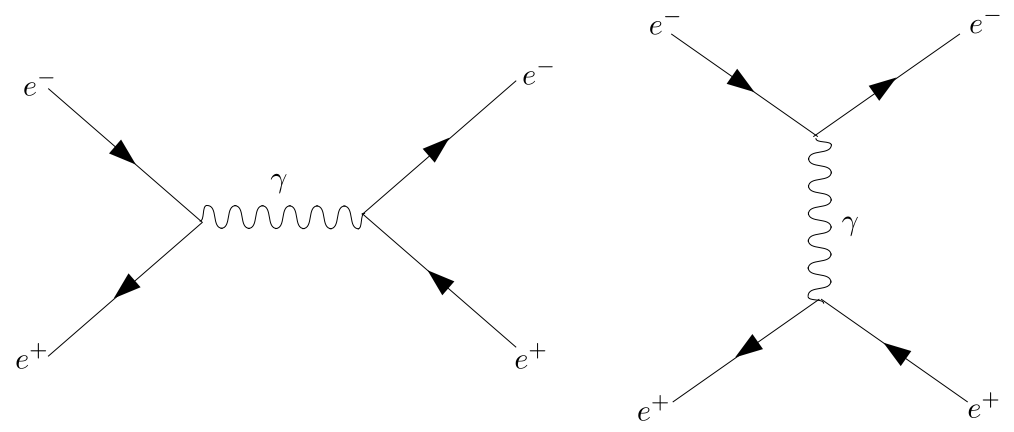
\includegraphics[scale=0.28]{Chapitre1/Images/bhabha.png} 
            \caption{Diffusion Bhabha en voie $s$ (gauche) et en voie $t$ (droite).}
        \label{bhabha}
        \end{figure}
        
        \section{Symétries et lois de conservation}

         En mécanique classique, il est facile de retrouver la seconde loi de Newton à partir du Lagrangien pour une particule classique se déplaçant selon l'axe $x$, défini comme la différence entre l'énergie cinétique et l'énergie potentielle :

        $$L=T-V=\frac{1}{2}m\dot{x}^2-V(x).$$

        En appliquant les équations d'Euler-Lagrange

        \begin{equation}
            \dv{t}\Biggl(\pdv{L}{\dot q_i}\Biggr)-\pdv{L}{q_i} = 0,
        \end{equation}

        on trouve alors pour la coordonnée généralisée $q_i=x$ :
        \begin{equation*}
        \begin{split}
            \quad \dv{t}\Biggl(\pdv{L}{\dot x}\Biggr)-\pdv{L}{x} & = \dv{t}m\dot x + \pdv{V}{x} \\
            & = 0.
        \end{split}
        \end{equation*}

        Soit finalement

        \begin{equation}
            m\ddot x = -\pdv{V(x)}{x}.
        \end{equation}

        Dans le cas d'une particule libre, c'est-à-dire lorsque $V(x)=0$, le Lagrangien ne contient plus de dépendance spatiale. Il comporte alors désormais une symétrie et devient invariant par transformation de translation de la coordonnée $x$ :

        $$x\rightarrow x' = x+\var x$$.

        Selon le théorème d'Emmy Noether introduit en 1915, la présence d'une symétrie au sein du Lagrangien entraîne l'existence d'une grandeur conservée au sein du système. Dans le cas où cette symétrie est une invariance par translation, il est possible de montrer que l'impulsion du système est conservée, illustrant notamment la 3ème loi de Newton. \\

        Par analogie, le formalisme de la mécanique lagrangienne s'inscrit naturellement au sein de la QFT afin de dériver les équations du mouvement satisfaites par les champs introduits plus tôt. La notion de Lagrangien pour un système discret peut être étendue à celle d'un système continu en introduisant une densité de Lagrangien et en remplaçant la dépendance aux coordonnées généralisées $(q_i,\dot q_i)$ par les champs $\phi_i$ et leurs dérivées selon les quatre dimensions de l'espace-temps $\partial_{\mu}\phi_i$ :

        $$L\Bigl(q_i,\dot q_i\Bigr)\rightarrow\mathcal{L}\Bigl(\phi_i,\partial_{\mu}\phi_i\Bigr),$$

        définie telle que 
        
        $$L\Bigl(\phi_i,\partial_{\mu}\phi_i\Bigr)=\int\mathcal{L}\Bigl(\phi_i,\partial_{\mu}\phi_i\Bigr)\dd[3]{x}.$$

        Enfin, l'action $S$ d'un système peut être définie comme l'intégrale temporelle du Lagrangien :

        $$S=\int L\Bigl(\phi_i,\partial_{\mu}\phi_i\Bigr)\dd{t} = \int\mathcal{L}\Bigl(\phi_i,\partial_{\mu}\phi_i\Bigr)\dd[4]{x},$$

        et selon le principe de moindre action, stipulant que l'action est stationnaire, il est possible de définir les équations d'Euler-Lagrange pour $\phi_i$ :

        \begin{equation}
        \boxed{
            \fdv{S}{\phi_i}=\pdv{\mathcal{L}}{\phi_i}-\partial_{\mu}\Biggl(\pdv{\mathcal{L}}{(\partial_{\mu}\phi_i)}\Biggr)=0.
        }
        \label{action}
        \end{equation}

        Prenons maintenant l'exemple de la densité de Lagrangien pour un spineur de Dirac libre en introduisant le spineur de Dirac adjoint $\overline{\psi}\equiv\psi^{\dag}\gamma^0$ :

        \begin{equation}
            \mathcal{L}_{\mbox{\tiny Dirac}}=\overline{\psi}\bigl(i\slashed\partial-m\bigr)\psi,
        \label{Ldirac}
        \end{equation}

        avec $\slashed \partial = \gamma^{\mu}\partial_{\mu}$. \\

        Il serait notamment possible de montrer que l'injection de $\mathcal{L}_{\mbox{\tiny Dirac}}$ dans l'équation \ref{action} permet de retrouver l'équation de Dirac telle que formulée dans l'équation \ref{dirac2}. Il est également possible de montrer que le Lagrangien de Dirac est invariant sous une transformation globale de $\psi$ du groupe de symétrie U($1$) telle que 

        $$\psi\rightarrow\psi'=e^{i\theta}\psi.$$

        Selon le théorème de Noether une nouvelle fois, cette symétrie implique l'existence d'une grandeur conservée qui peut être montrée comme étant le quadrivecteur constitué de la densité et du courant de probabilité définis dans \ref{probdirac} : 

        \begin{equation}
        \boxed{
            j^{\mu}=(\rho,\vb{j})=\overline{\psi}\gamma^{\mu}\psi. 
        }
        \label{fermioncurrent}
        \end{equation}

        \vspace{10pt}
        En résumé, les physiciens sont parvenus en près de 50 ans à mettre au point des outils permettant d'étudier et de comprendre le fonctionnement de l'infiniment petit. Ces recherches ont notamment permis de nombreuses découvertes qui représentent aujourd'hui les fondements de la physique des particules moderne. La théorie quantique de l'électromagnétisme, aboutie entre 1946 et 1950 par R. Feynman, J. Schwinger et S. Tomonaga, est encore aujourd'hui une théorie dont la précision des prédictions reste inégalée. Cette période marque aussi le commencement de nombreux travaux dans le but de développer des nouveaux modèles dans le cadre de la théorie quantique des champs qui constitueront les prémices du modèle standard de la physique des particules. Le chapitre suivant sera consacré à la mise en forme et à l'assemblage des différentes théories qui le constituent, en s'appuyant sur des principes de symétrie tels qu'ils ont été présentés dans la dernière partie de ce chapitre.